%!TEX program = xelatex
\documentclass[dvipsnames, svgnames,a4paper,11pt]{article}
% ----------------------------------------------------
%   中山大学物理与天文学院本科实验报告模板
%   作者:Huanyu Shi,2019级
%   知乎:https://www.zhihu.com/people/za-ran-zhu-fu-liu-xing
%   Github:https://github.com/Huanyu-Shi/SYSU-SPA-Labreport-Template
%   Last update : 2023.4.10
% ----------------------------------------------------

% ----------------------------------------------------- 
%	加边框的命令
%	参考:https://tex.stackexchange.com/questions/531559/how-to-add-the-page-border-for-first-two-pages-in-latex
\usepackage{tikz}
\usetikzlibrary{calc}
\usepackage{eso-pic}
\AddToShipoutPictureBG{%
\begin{tikzpicture}[overlay,remember picture]
\draw[line width=0.6pt] % 边框粗细
    ($ (current page.north west) + (0.6cm,-0.6cm) $)
    rectangle
    ($ (current page.south east) + (-0.6cm,0.6cm) $); % 边框位置
\end{tikzpicture}}


\usepackage{xcolor}
\definecolor{c1}{HTML}{2752C9} % 目录颜色
\definecolor{c2}{RGB}{190,20,83} % 引用颜色

\usepackage{ctex}
\usepackage[top=28mm,bottom=28mm,left=15mm,right=15mm]{geometry}
\usepackage{hyperref} 
\hypersetup{
	colorlinks,
	linktoc = section, % 超链接位置,选项有section, page, all
	linkcolor = c1, % linkcolor 目录颜色
	citecolor = c1  % citecolor 引用颜色
}
\usepackage{amsmath,enumerate,multirow,float}
\usepackage{tabularx}
\usepackage{tabu}
\usepackage{subfig}
\usepackage{fancyhdr}
\usepackage{graphicx}
\usepackage{wrapfig}  
\usepackage{physics}
\usepackage{appendix}
\usepackage{amsfonts}

%
\usepackage{tcolorbox}
\tcbuselibrary{skins,breakable}
\newtcolorbox{tbox}[2][]{
    colframe=black!70!,
    breakable,
    enhanced,
	boxrule =0.5pt,
    title = {#2},
    fonttitle = \large\kaishu\bfseries,
	drop fuzzy shadow,
    #1
}
\newtcolorbox[auto counter,number within=section]{question}[1][]{
  top=2pt,bottom=2pt,arc=1mm,
  boxrule=0.5pt,
%   frame hidden,
  breakable,
  enhanced, %跨页后不会显示下边框
  coltitle=c1!80!gray,
  colframe=c1,
  colback=c1!3!white,
  drop fuzzy shadow,
  title={思考题~\thetcbcounter:\quad},
  fonttitle=\bfseries,
  attach title to upper,
  #1
}
\newcommand{\setLhead}[1]{%
  \lhead{{\color{gray}\kaishu #1}} % 定义新的命令,设置右边页眉的内容
}
\newcommand{\setRhead}[1]{%
  \rhead{{\color{gray}\kaishu #1}} % 定义新的命令,设置右边页眉的内容
}
% ---------------------------------------------------------------------
%	利用cleveref改变引用格式,\cref是引用命令
\usepackage{cleveref}
\crefformat{figure}{#2{\textcolor{c2}{图 #1}}#3} % 图片的引用格式
\crefformat{equation}{#2{(\textcolor{c2}{#1})}#3} % 公式的引用格式
\crefformat{table}{#2{\textcolor{c2}{表 #1}}#3} % 表格的引用格式


% ---------------------------------------------------------------------
%	页眉页脚设置
\fancypagestyle{plain}{\pagestyle{fancy}}
\pagestyle{fancy}
\setLhead{中山大学物理与天文学院基础物理实验预习报告}
%\lhead{\kaishu 中山大学物理与天文学院物理实验\uppercase\expandafter{\romannumeral3}} % 左边页眉,学院 + 课程
%\rhead{{\color{gray}\kaishu Template 实验报告模板}} % 右边页眉,实验报告标题
\setRhead{实验1\hspace{1pt}冰的熔化热测量}
\cfoot{\thepage} % 页脚,中间添加页码


% ---------------------------------------------------------------------
%	对目录、章节标题的设置
\renewcommand{\contentsname}{\centerline{\huge 目录}}
\usepackage{titlesec}
\usepackage{titletoc}
% \titleformat{章节}[形状]{格式}{标题序号}{序号与标题间距}{标题前命令}[标题后命令]
\titleformat{\section}{\centering\LARGE\songti}{}{1em}{}

% ---------------------------------------------------------------------
%   listing代码环境设置
\usepackage{listings}
\lstloadlanguages{python}
\lstdefinestyle{pythonstyle}{
backgroundcolor=\color{gray!5},
language=python,
frameround=tftt,
frame=shadowbox, 
keepspaces=true,
breaklines,
columns=spaceflexible,                   
basicstyle=\ttfamily\small, % 基本文本设置,字体为teletype,大小为scriptsize
keywordstyle=[1]\color{c1}\bfseries, 
keywordstyle=[2]\color{Red!70!black},   
stringstyle=\color{Purple},       
showstringspaces=false,
commentstyle=\ttfamily\scriptsize\color{green!40!black},%注释文本设置,字体为sf,大小为smaller
tabsize=2,
morekeywords={as},
morekeywords=[2]{np, plt, sp},
numbers=left, % 代码行数
numberstyle=\it\tiny\color{gray}, % 代码行数的数字字体设置
stepnumber=1,
rulesepcolor=\color{gray!30!white}
}




% ---------------------------------------------------------------------
%	其他设置
\def\degree{${}^{\circ}$} % 角度
\graphicspath{{./images/}} % 插入图片的相对路径
\allowdisplaybreaks[4]  %允许公式跨页 % 导入模板的相关设置
\usepackage{lipsum}
\usepackage{indentfirst}
\usepackage{pdfpages}
\usepackage{multirow}
\usepackage{subfig}
\usepackage{graphicx}
\usepackage{float} 
\usepackage{booktabs}
\usepackage{enumerate}
\usepackage{makecell} 
\renewcommand{\d}{\mathrm{d}}
\newcommand{\upcite}[1]{\textsuperscript{\textsuperscript{\cite{#1}}}}


%---------------------------------------------------------------------
%	正文
%---------------------------------------------------------------------
\setRhead{薄透镜焦距的测量}%实验名称
\begin{document}


\begin{table}
	\renewcommand\arraystretch{1.7}
	\begin{tabularx}{\textwidth}{
		|X|X|X|X
		|X|X|X|X|}
	\hline
	\multicolumn{2}{|c|}{预习报告}&\multicolumn{2}{|c|}{实验记录}&\multicolumn{2}{|c|}{分析讨论}&\multicolumn{2}{|c|}{总成绩}\\
	\hline
	 & &  & &  & &  & \\
	\hline
	\end{tabularx}
\end{table}


\begin{table}
	\renewcommand\arraystretch{1.7}
	\begin{tabularx}{\textwidth}{|X|X|X|X|}
	\hline
	专业:& 物理学类 &年级:& 2023级\\
	\hline
	姓名:& 姚昊廷  & 学号:&22322091\\
	\hline
	实验时间:& 2024.12.19& 教师签名:& \\
	\hline
	\end{tabularx}
\end{table}

\begin{center}
	\LARGE 薄透镜焦距的测量
\end{center}

\textbf{【实验报告注意事项】}
\begin{enumerate}
	\item 实验报告由三部分组成:
	\begin{enumerate}
		\item 预习报告:(提前一周)认真研读\underline{\textbf{实验讲义}},弄清实验原理;实验所需的仪器设备、用具及其使用(强烈建议到实验室预习),完成课前预习思考题;了解实验需要测量的物理量,并根据要求提前准备实验记录表格(第一循环实验已由教师提供模板,可以打印)。预习成绩低于10分(共20分)者不能做实验。
	    \item 实验记录:认真、客观记录实验条件、实验过程中的现象以及数据。实验记录请用珠笔或者钢笔书写并签名(\textcolor{red}{\textbf{用铅笔记录的被认为无效}})。\textcolor{red}{\textbf{保持原始记录,包括写错删除部分,如因误记需要修改记录,必须按规范修改。}}(不得输入电脑打印,但可扫描手记后打印扫描件);离开前请实验教师检查记录并签名。
	    \item 分析讨论:处理实验原始数据(学习仪器使用类型的实验除外),对数据的可靠性和合理性进行分析;按规范呈现数据和结果(图、表),包括数据、图表按顺序编号及其引用;分析物理现象(含回答实验思考题,写出问题思考过程,必要时按规范引用数据);最后得出结论。
	\end{enumerate}
	\textbf{实验报告就是将预习报告、实验记录、和数据处理与分析合起来,加上本页封面。}
	\item 每次完成实验后的一周内交\textbf{实验报告}(特殊情况不能超过两周)。
	\item 除实验记录外,实验报告其他部分建议双面打印。
\end{enumerate}

\textbf{【实验安全与实验室注意事项】}\\
\begin{enumerate}
    \item 实验中需带手套,尽量避免用手直接接触镜片的光学面。若不小心触摸了光学表面,需尽快用镜头纸或擦镜布擦拭干净。
    \item 安装镜片时需在光学平台上尽量靠近台面的高度操作,以免失手跌落摔碎镜片。
    \item 实验平台配件所用固定螺钉需拧紧,以免镜架晃动;但不可过紧,以免损坏。
    \item 实验前需按仪器清单检查光学元件是否齐全,实验结束后按照顺序放回元件盒。
\end{enumerate}

\clearpage
\tableofcontents
\clearpage

\setcounter{section}{0}
\section{薄透镜焦距的测量\ \textbf{预习报告}}
	
\subsection{实验目的}
\begin{enumerate}
    \item 熟悉光具座及其附件的使用。
	\item 通过实验进一步理解薄透镜的成像规律。
	\item 掌握利用自准直方法测量薄透镜焦距。
	\item 掌握和理解光学系统共轴等高调节的方法。
\end{enumerate}
\subsection{仪器用具}
\begin{table}[htbp]
	\centering
	\renewcommand\arraystretch{1.6}
	% \setlength{\tabcolsep}{10mm}
	\begin{tabular}{p{0.05\textwidth}|p{0.20\textwidth}|p{0.05\textwidth}|p{0.5\textwidth}}
	\hline
	编号& 仪器用具名称 & 数量 &  主要参数(型号,测量范围,测量精度等) \\
	\hline
	1&透镜LC&1 &\\
	\hline
	2&白光光源&1&GY-6 型,亮度可调,即溴钨灯\\
	\hline
	3&白屏&1&SZ-13\\
	\hline
    4&物屏&1&SZ-14\\
	\hline
    5&透镜L&1&f=150mm 等\\
	\hline
    6&透镜架&1&SZ-14\\
	\hline
    7&平面镜&1&$\Phi36*4$\\
	\hline
    8&透镜架&1&SZ-14\\
	\hline
    9-12&平移底座&4&\\
	\hline
\end{tabular}
\end{table}


\subsection{原理概述和实验前思考题}
\begin{question}
    什么是透镜的“焦点”、“焦距”和“焦平面”?会聚透镜和发散透镜的区别?什么情况下透镜的像方焦距等于透镜的物方焦距?
    \tcblower
    薄透镜是指厚度远小于焦距,也远小于球面曲率半径的透镜,是光学仪器中最常用的光
学元件之一. 透镜一般采用光学玻璃制作,具有两个折射面. 若折射面是球面的一部分则称为
球面透镜,若不是球面则称为非球面透镜.透镜折射面形状通常有凸球面、凹球面和平面三
种,可组成双凸、平凸、正弯月、双凹、平凹、负弯月六种形状的透镜.前三种透镜使入射
的平行光会聚,像方焦距为正值,称为会聚透镜(或正透镜) ;后三种透镜使入射的平行光发
散,像方焦距为负值,称为发散透镜(或负透镜) .平行光束通过薄透镜后的会聚点称为焦点,从焦点到透镜光心的距离
称为焦距 .在理想情况下,即透镜完全对称,透镜两端环境也完全对称,光线通过透镜或球面镜后,会汇聚到焦点上,即物方焦距与像方焦距相等.
\end{question}

\begin{question}
    本实验的误差主要来源,如何减小误差?
    \tcblower
    所成像并非等大倒立或所得光斑并非最小导致所得距离并非焦距。多次移动改变距离,多次得到焦距取平均值。
\end{question}

\begin{question}
    采用三条基本光线绘图的方法画出自准法测量薄透镜焦距的实验原理光路图(提示:注意“焦平面”的含义,可参考《基础物理实验》(沈韩编著)P238)
    \tcblower
    \begin{figure}[H]
        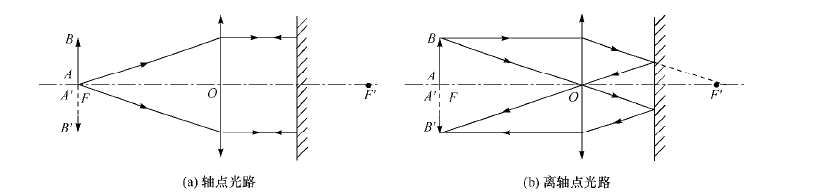
\includegraphics[width=\textwidth]{透镜焦距光路图.png}
    \end{figure}
\end{question}

\clearpage
\setLhead{中山大学物理与天文学院基础物理实验记录}
\begin{table}
	\renewcommand\arraystretch{1.7}
	\centering
	\begin{tabularx}{\textwidth}{|X|X|X|X|}
	\hline
	专业:& 物理学类 &年级:& 2023级 \\
	\hline
	姓名: &姚昊廷& 学号:&22322091  \\
	\hline
	室温:&$22^\circ$C&实验地点:&A508  14\\
	\hline
	学生签名:& & 评分: &\\
	\hline
	实验时间:& 2024.12.19& 教师签名:&\\
	\hline
	\end{tabularx}
\end{table}
\section{薄透镜焦距的测量\ \textbf{实验记录}}
\subsection{实验内容、步骤、结果}
\subsubsection{简单测量会聚透镜的焦距}
\begin{enumerate}
	\item 摆好光路图,调节光学元件等高共轴
	\item 以溴钨灯白光源为物,放置在尽可能远处,通过透镜形成一个实焦点
	\item 测量记录透镜物方焦距7次
\end{enumerate}
\begin{table}[H]
	\centering
	\caption{简单测量会聚透镜焦距}
	\begin{tabular}{cc}
		\toprule
		测量次序&透镜物方焦距/cm\\
		\midrule
		1&17.60\\
		2&17.70\\
		3&17.65\\
		4&17.75\\
		5&17.70\\
		6&17.65\\
		7&17.70\\
		\toprule
	\end{tabular}
\end{table}
反转透镜,再次测量记录透镜像方焦距
\begin{table}[H]
	\centering
	\begin{tabular}{cc}
		\toprule
		测量次序&透镜像方焦距/cm\\
		\midrule
		1&17.15\\
		2&17.32\\
		3&17.15\\
		4&17.35\\
		5&17.20\\
		6&17.22\\
		7&17.25\\
		\toprule
	\end{tabular}
\end{table}
\subsubsection{自准法测会聚透镜的焦距}
\begin{enumerate}
	\item 摆好光路,将物屏摆在光源前;调节各元件等高共轴。
	\item 移动透镜,简单描述如何判断物屏所在位置即透镜焦距?并测量记录物屏和透镜的位置A1,A2各7次。
\end{enumerate}
依照光路图搭建好光路,调节各元件等高共轴,随后调整透镜位置直至物屏上出现的光斑与原来孔位组成一个完整圆周,此时便可判断物屏与透镜所隔距离便是透镜焦距。
\begin{table}[H]
	\centering
	\caption{自准法测会聚透镜焦距}
	\begin{tabular}{ccc}
		\toprule
		测量次序&物屏位置A1/cm&透镜位置A2/cm\\
		\midrule
		1&65.85&81.60\\
		2&65.85&81.55\\
		3&65.85&81.90\\
		4&65.85&81.85\\
		5&65.85&81.88\\
		6&65.85&81.95\\
		7&65.85&81.90\\
		\toprule
	\end{tabular}
\end{table}
反转透镜,做必要的调节,再测量记录物屏和透镜的位B1,B2各五次。
\begin{table}[H]
	\centering
	\caption{自准法测会聚透镜焦距}
	\begin{tabular}{ccc}
		\toprule
		测量次序&物屏位置B1/cm&透镜位置B2/cm\\
		\midrule
		1&65.85&82.40\\
		2&65.85&82.45\\
		3&65.85&82.30\\
		4&65.85&82.10\\
		5&65.85&82.20\\
		6&65.85&82.35\\
		7&65.85&82.38\\
		\toprule
	\end{tabular}
\end{table}
\subsubsection{透镜焦距确定之后,改变平面镜与透镜之间的距离,描述物屏上观察的现象。}
移动平面镜,当平面镜靠近透镜时,物屏上实像变小变亮,在最靠近透镜处略微变小。远离透镜实像在一定距离后迅速变小且变暗,在极大
距离处会形成微亮实像面积较大,出现在物屏四周,形状类似一开始的实像。
\subsubsection{实验过程遇到问题记录}
\begin{enumerate}
	\item 由于没有标注,确定各镜片位置较难。
	\item 实验装置长度有限,无法很好达到平行光条件。
\end{enumerate}

\clearpage
\setLhead{中山大学物理与天文学院基础物理实验分析与讨论}
\begin{table}
	\renewcommand\arraystretch{1.7}
	\begin{tabularx}{\textwidth}{|X|X|X|X|}
	\hline
	专业:& 物理学 &年级:& 2023级\\
	\hline
	姓名: &姚昊廷& 学号:&22322091 \\
	\hline
    日期:&2024.12.19 & 评分: &\\
	\hline
	\end{tabularx}
\end{table}

\section{薄透镜焦距的测量\ \textbf{分析与讨论}}
\subsection{给出简单测量法测得的会聚透镜的物方焦距和像方焦距和相应的误差(分析), 并分析测量值与理论值的差别和原因。}
\textbf{物方焦距}:均值为$\overline{f}=\sum_{i=1}^{7}\frac{f_i}{7}=17.68$cm,标准差为$\sigma=\sqrt{\frac{\sum_{i=1}^{7}(f_i-\overline{f})^2}{7-1}}=0.049$cm,则
A类不确定度为$u_a=\frac{\sigma}{\sqrt{7}}=0.019$cm,B类不确定度为$u_B=\frac{0.1cm}{\sqrt{3}}=0.0058$cm
自由度为$\nu_A=n-1=6$,取置信概率为$95\%$,查表知$t=2.45$故$u_f=\sqrt{t^2u_A^2+u_B^2}=0.047$cm。
故测量结果为
\begin{align*}
	f=\overline{f}\pm u_f=(17.68\pm0.05)\text{cm}
\end{align*}\par

\textbf{像方焦距}:均值为$\overline{f}=\sum_{i=1}^{7}\frac{f_i}{7}=17.23$cm,标准差为$\sigma=\sqrt{\frac{\sum_{i=1}^{7}(f_i-\overline{f})^2}{7-1}}=0.08$cm,则
A类不确定度为$u_a=\frac{\sigma}{\sqrt{7}}=0.03$cm,B类不确定度为$u_B=\frac{0.1cm}{\sqrt{3}}=0.0058$cm
自由度为$\nu_A=n-1=6$,取置信概率为$95\%$,查表知$t=2.45$故$u_f=\sqrt{t^2u_A^2+u_B^2}=0.073$cm。
故测量结果为
\begin{align*}
	f=\overline{f}\pm u_f=(17.23\pm0.07)\text{cm}
\end{align*}

两测量结果均大于15cm,误差来源可能是光源距离透镜过近导致不满足平行条件。
\subsection{给出自准法测得的会聚透镜的物方焦距和像方焦距和相应的误差(分析)。}
\begin{table}[H]
	\centering
	\begin{tabular}{ccc}
		\toprule
		测量次序&物方焦距/cm&像方焦距/cm\\
		\midrule
		1&15.75&16.55\\
		2&15.70&16.60\\
		3&16.05&16.45\\
		4&16.00&16.25\\
		5&16.03&16.35\\
		6&16.10&16.50\\
		7&16.05&16.53\\
		\toprule
	\end{tabular}
\end{table}
\textbf{物方焦距}:均值为$\overline{f}=\sum_{i=1}^{7}\frac{f_i}{7}=15.95$cm,标准差为$\sigma=\sqrt{\frac{\sum_{i=1}^{7}(f_i-\overline{f})^2}{7-1}}=0.16$cm,则
A类不确定度为$u_a=\frac{\sigma}{\sqrt{7}}=0.06$cm,B类不确定度为$u_B=\frac{0.1cm}{\sqrt{3}}=0.0058$cm
自由度为$\nu_A=n-1=6$,取置信概率为$95\%$,查表知$t=2.45$故$u_f=\sqrt{t^2u_A^2+u_B^2}=0.15$cm。
故测量结果为
\begin{align*}
	f=\overline{f}\pm u_f=(15.95\pm0.15)\text{cm}
\end{align*}\par

\textbf{像方焦距}:均值为$\overline{f}=\sum_{i=1}^{7}\frac{f_i}{7}=16.46$cm,标准差为$\sigma=\sqrt{\frac{\sum_{i=1}^{7}(f_i-\overline{f})^2}{7-1}}=0.12$cm,则
A类不确定度为$u_a=\frac{\sigma}{\sqrt{7}}=0.05$cm,B类不确定度为$u_B=\frac{0.1cm}{\sqrt{3}}=0.0058$cm
自由度为$\nu_A=n-1=6$,取置信概率为$95\%$,查表知$t=2.45$故$u_f=\sqrt{t^2u_A^2+u_B^2}=0.12$cm。
故测量结果为
\begin{align*}
    f=\overline{f}\pm u_f=(16.46\pm0.12)\text{cm}
\end{align*}\par


两测量结果均大于15cm,误差来源可能是光源距离透镜过近导致不满足平行条件以及读数误差。
\subsection{实验后思考题}
\begin{question}
	本实验中测量薄透镜焦距时,为什么需要将透镜旋转180度再测量?
	\tcblower
	透镜制造受制于精度限制,无法达到完全对称,因此透镜两面焦距不同。
\end{question}
\clearpage
% ---------------------------------------------------------------------
%   参考文献
%   注:使用参考文献时应按照xelatex->bibtex->xelatex->xelatex顺序进行编译
%\phantomsection
%\addcontentsline{toc}{section}{参考文献}
%\bibliographystyle{unsrt}
%\bibliography{myref}
%\begin{thebibliography}{9}
%	\bibitem{ref1} 沈雨欣,翁存程,蒋丽钦.双棱镜干涉法准确测量钠光波长[J].大学物理实验,2023,36(03):40-43.DOI:10.14139/j.cnki.cn22-1228.2023.03.008.
%	\bibitem{ref2} 牟泉润,孙丽媛,杜月棋,等.基于干涉原理的光波长测量装置设计[J].大学物理实验,2021,34(06):80-83+89.DOI:10.14139/j.cnki.cn22-1228.2021.06.018.
%	\bibitem{ref3} 王仁洲,杨涛.一种用激光干涉测量光波波长的新方法[J].大学物理实验,2014,27(06):41-43.DOI:10.14139/j.cnki.cn22-1228.2014.06.014.
%\end{thebibliography}


%\clearpage
\appendix
\appendixpage
\addappheadtotoc
%\subsection*{相图代码}
%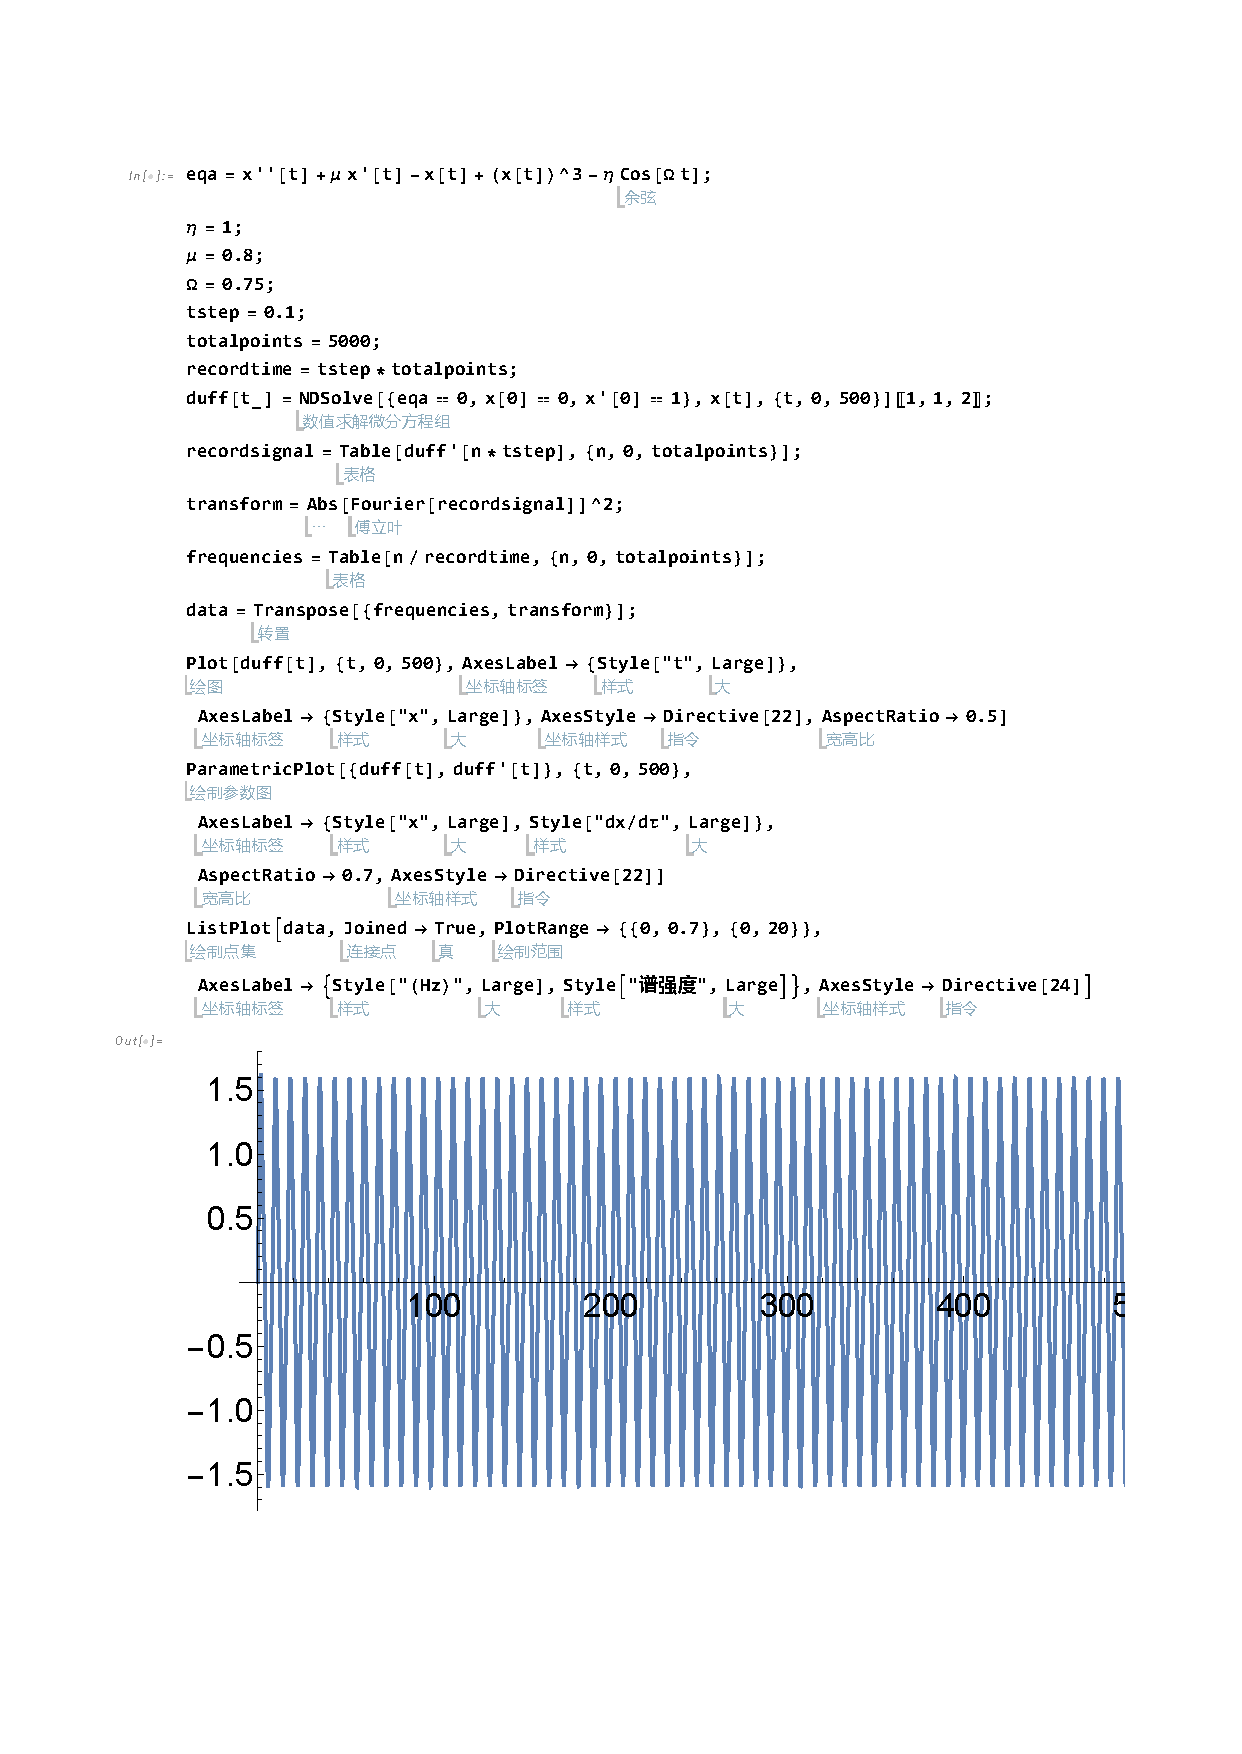
\includepdf[pages=-]{chaos.pdf}
\subsection*{原件}
%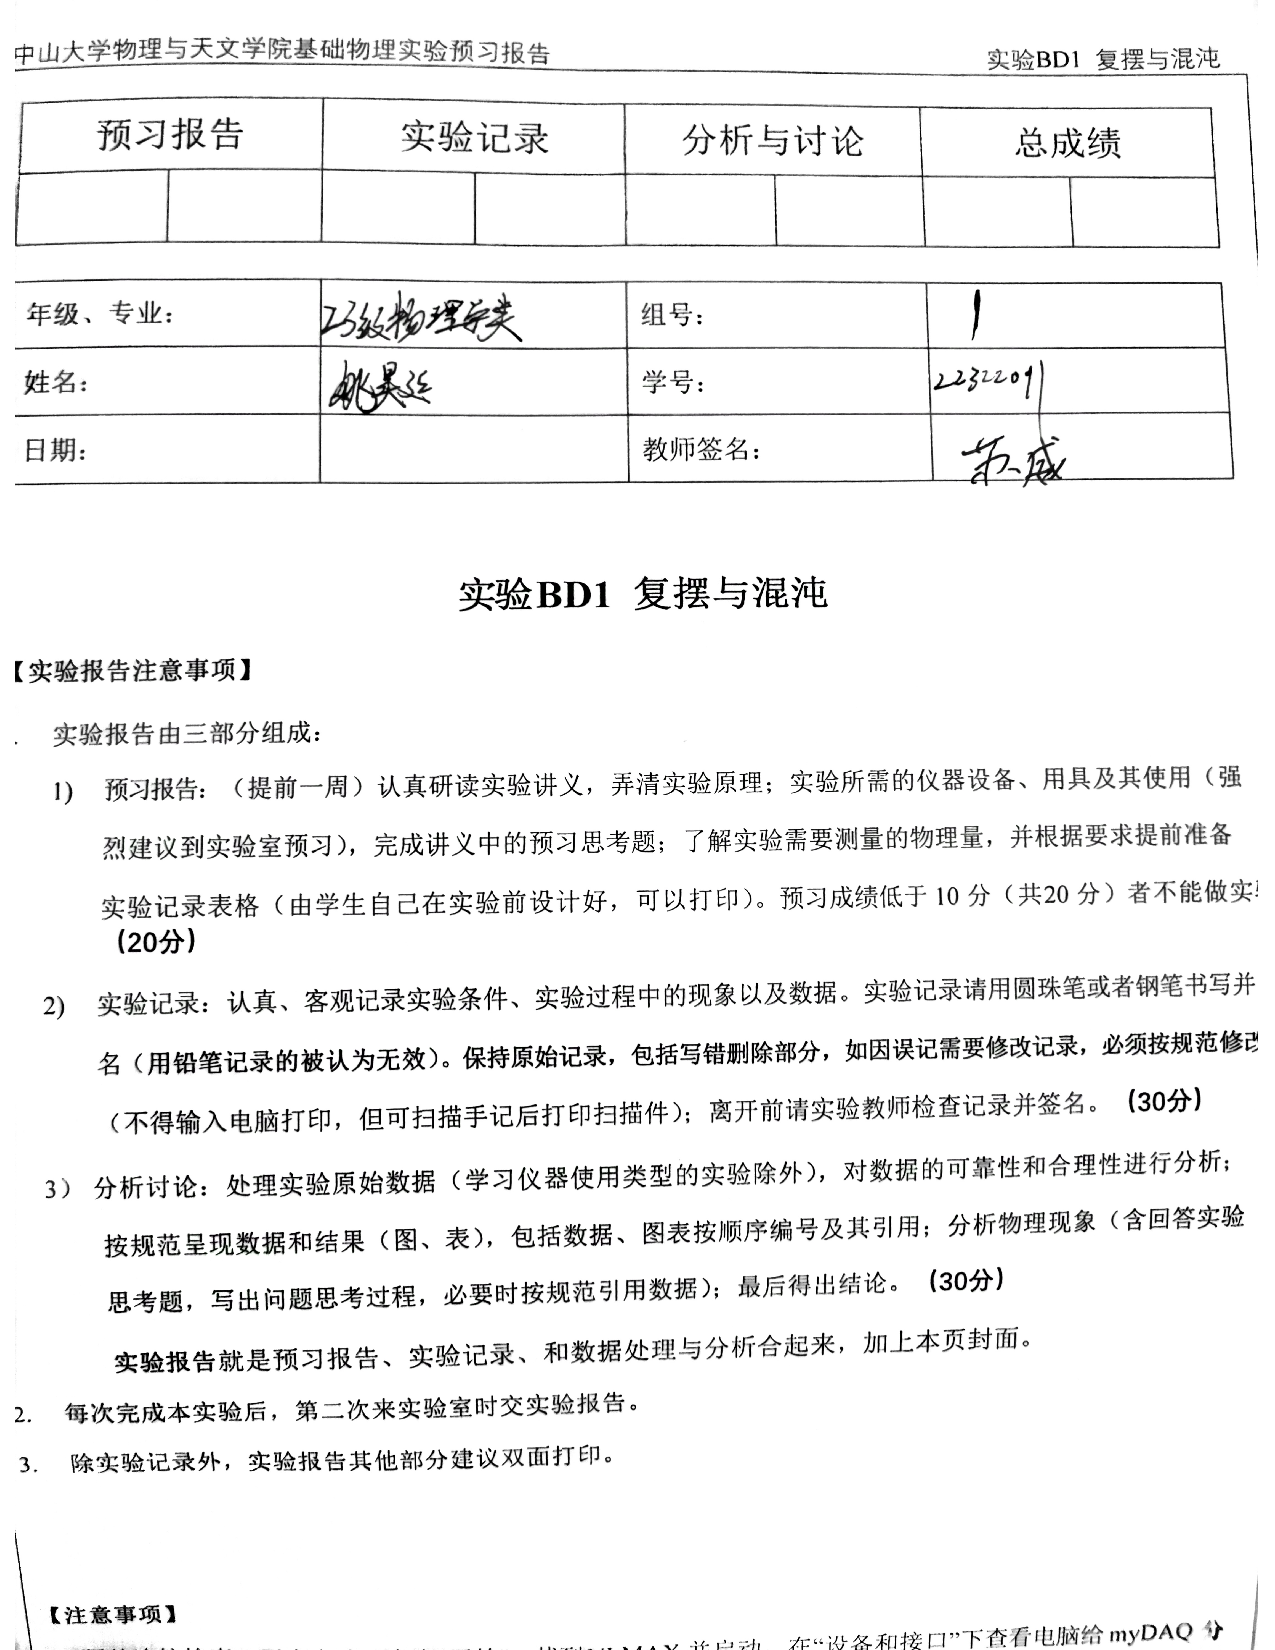
\includepdf[pages=-]{实验3原件.pdf}
\begin{figure}[H]
	\centering
	\includegraphics[width=\textwidth]{焦距数据.jpg}
	
\end{figure}
\begin{figure}[H]
	\centering
	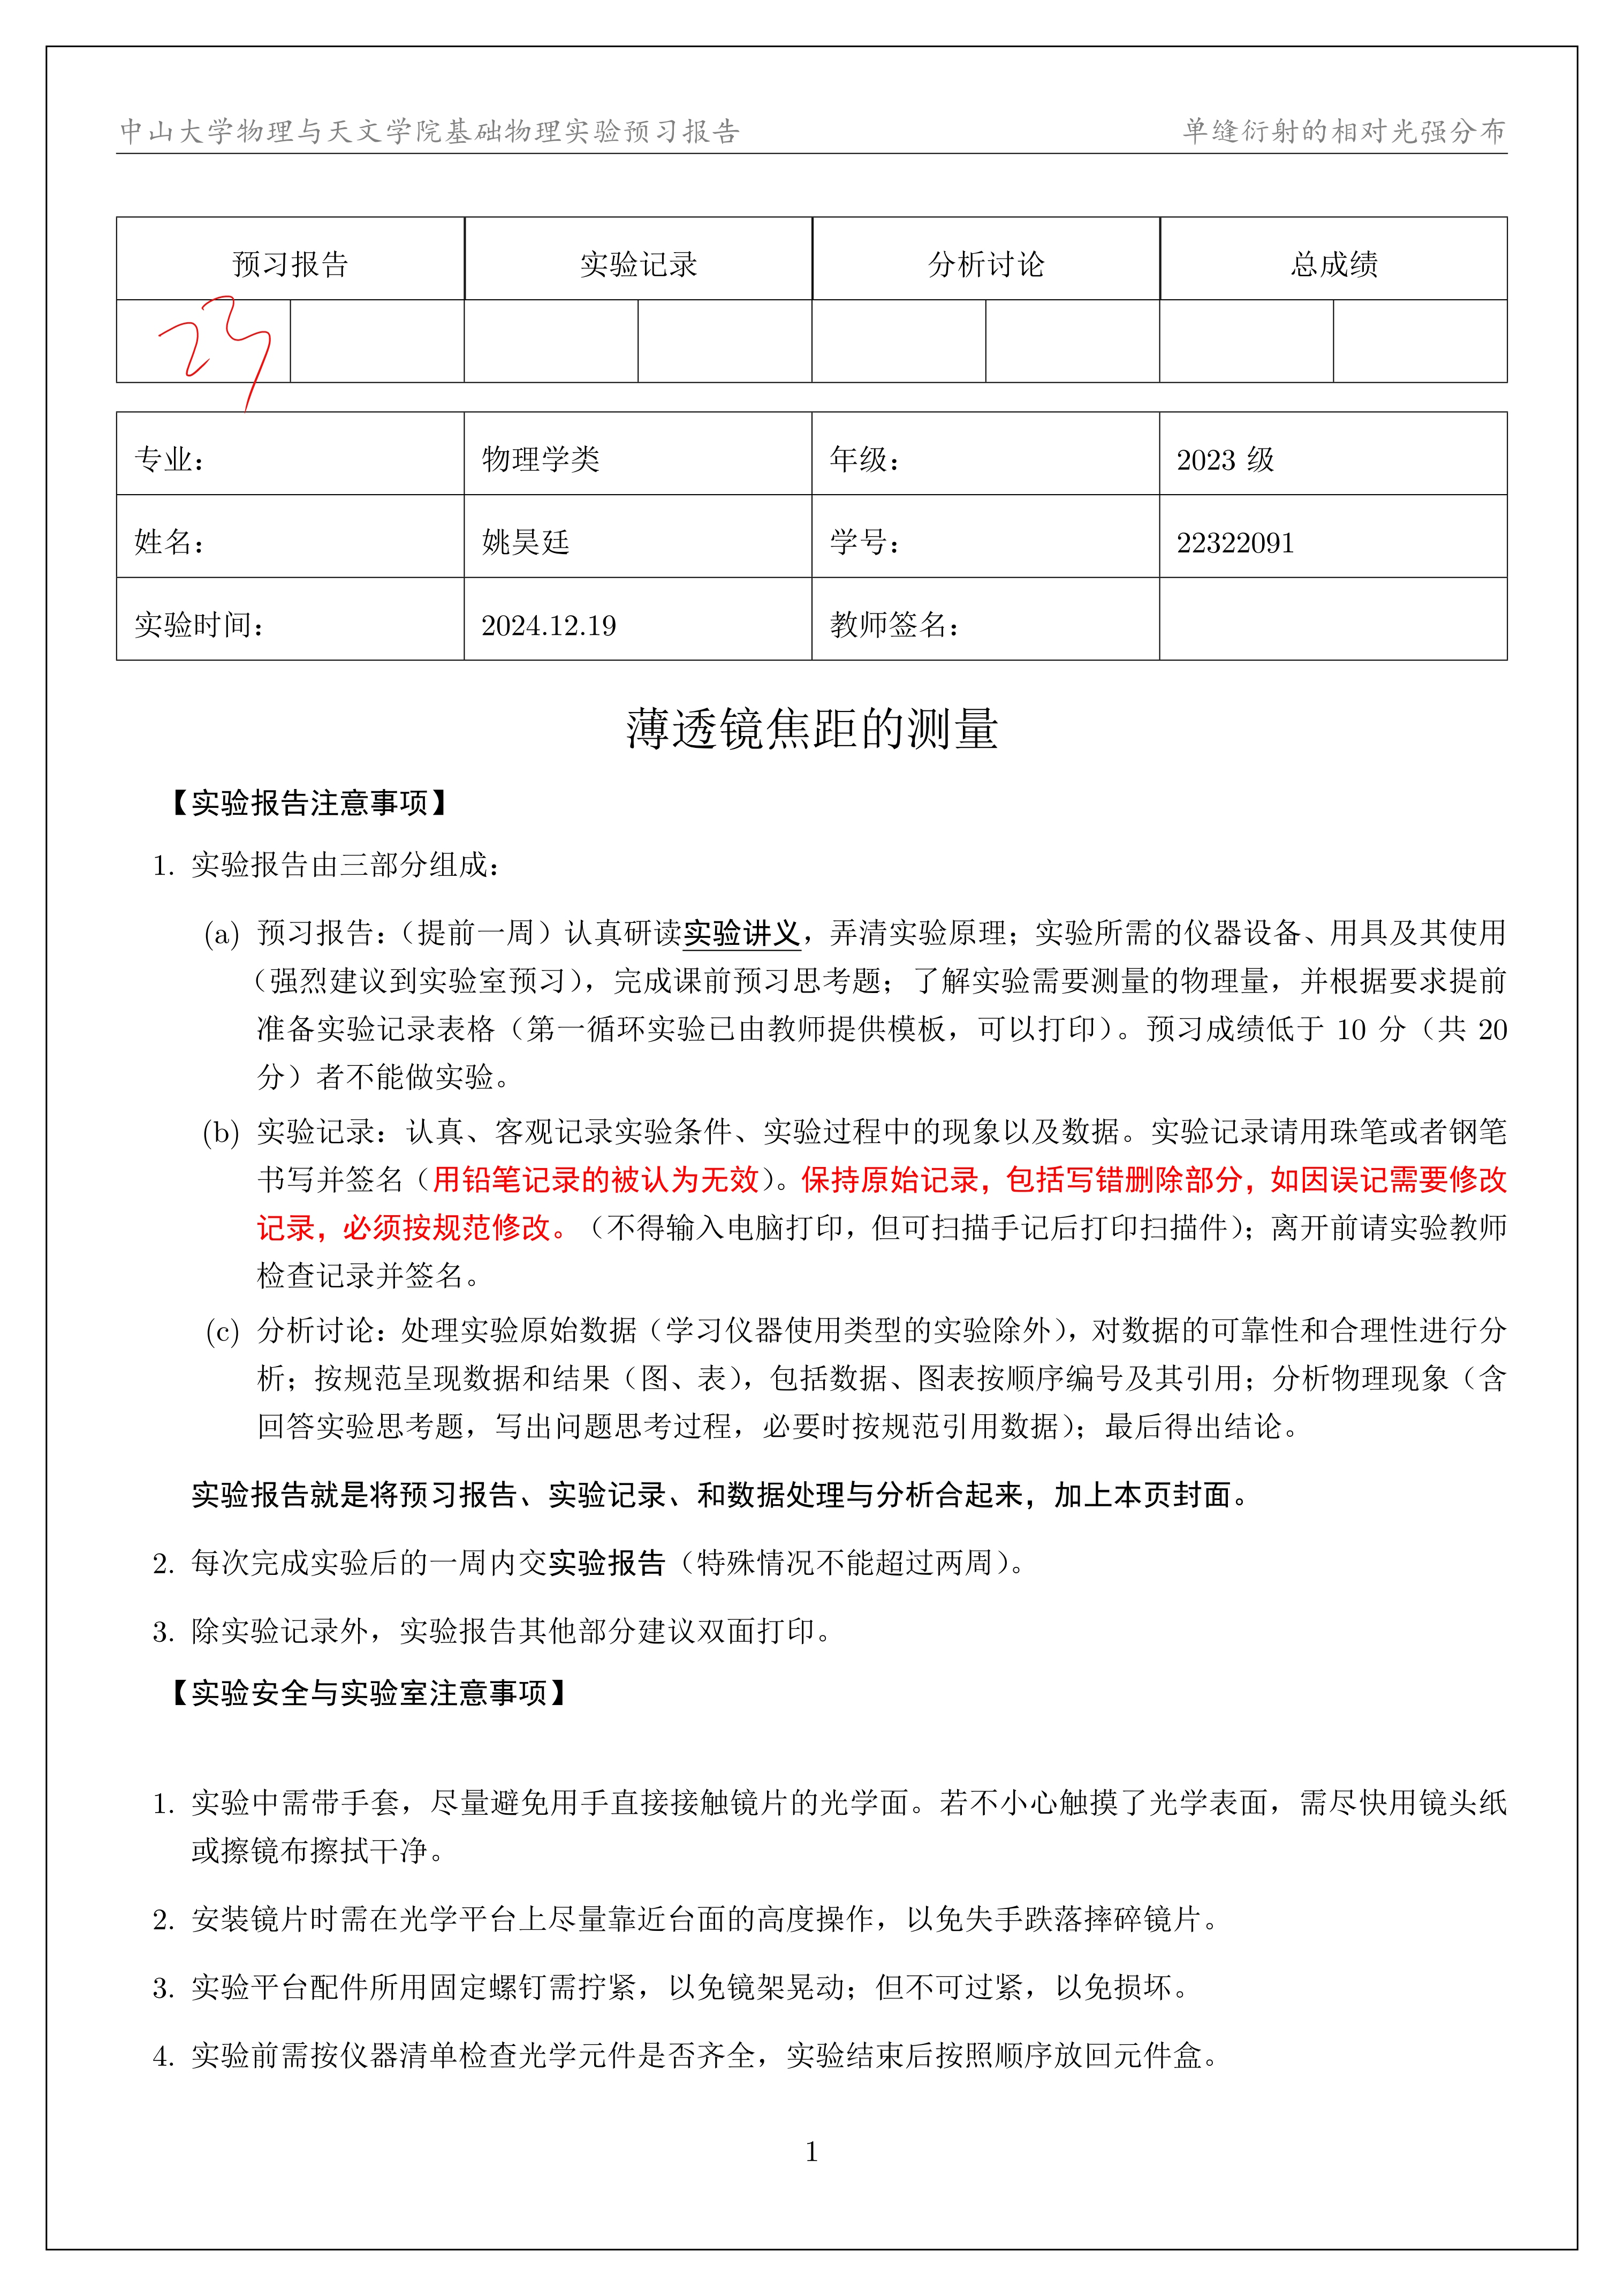
\includegraphics[width=\textwidth]{透镜焦距.jpg}
	
\end{figure}

%\begin{figure}[H]
%	\centering
%	\includegraphics[width=0.4\textwidth]{单缝原件1.jpg}
%	\includegraphics[width=0.4\textwidth]{单缝原件2.jpg}
%	\includegraphics[width=0.4\textwidth]{单缝原件3.jpg}
%	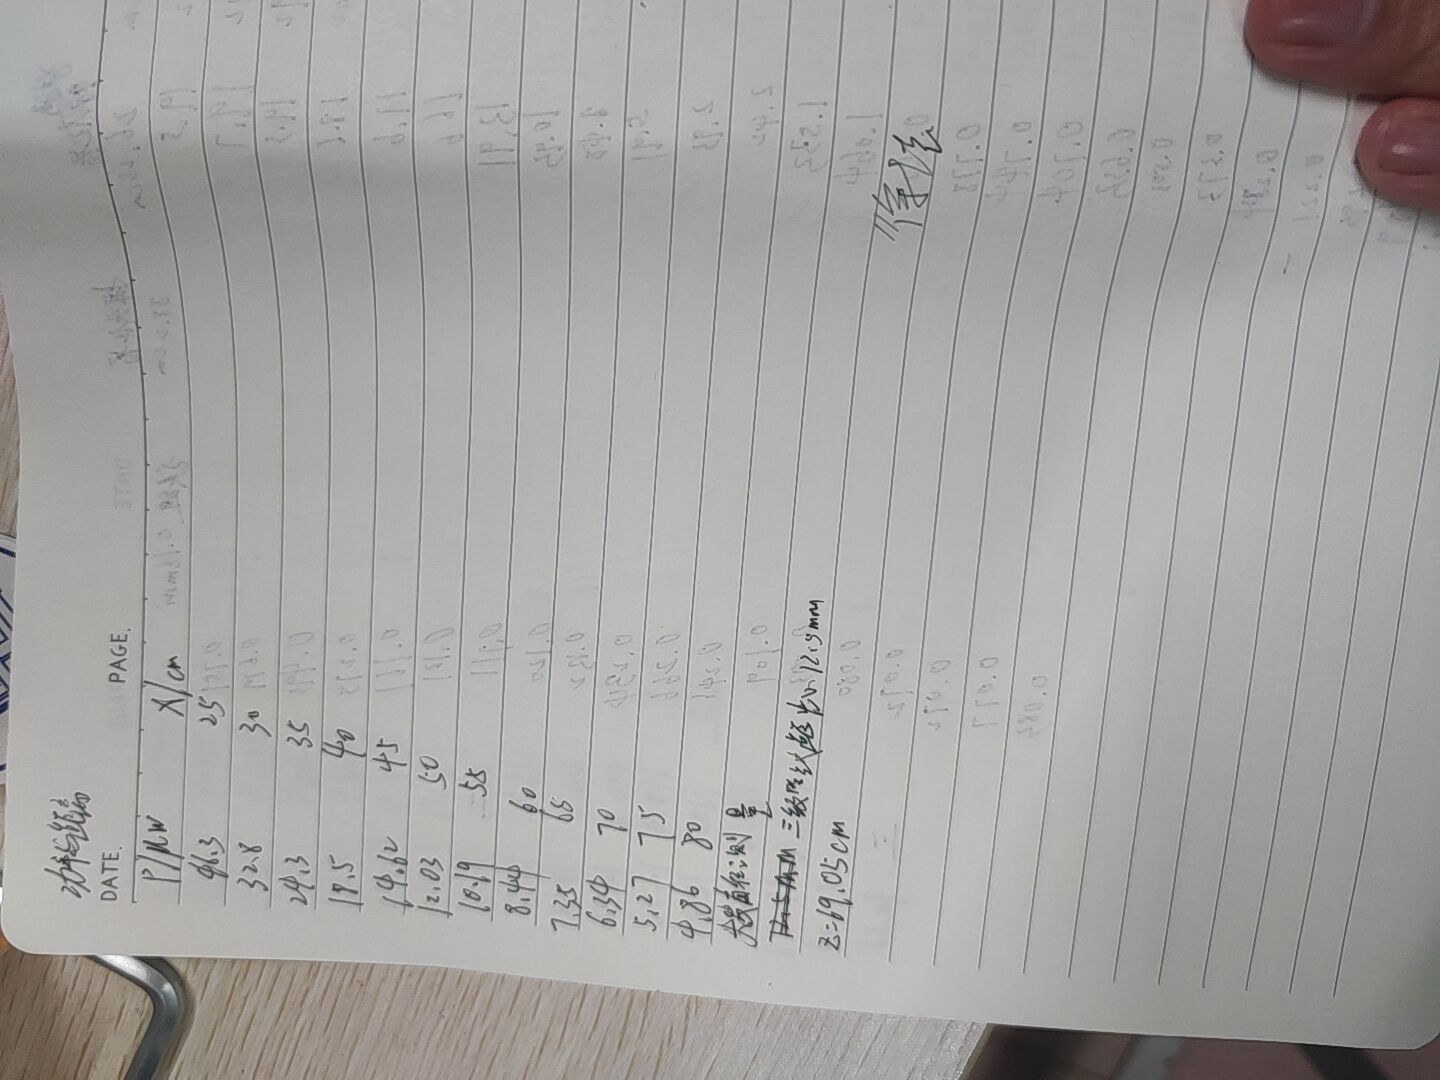
\includegraphics[width=0.4\textwidth]{单缝原件4.jpg}
%\end{figure}
\subsection*{桌面}
\begin{figure}[H]
	\includegraphics[width=0.95\textwidth]{焦距桌面.jpg}
\end{figure}
\end{document}
%